\documentclass[aspectratio=169,11pt,svgnames]{beamer}

\usepackage[english]{babel}
\usepackage{graphicx}
\usepackage{enumitem}
\usepackage{amsmath}
\usepackage{mathtools}
\usepackage{float}
\usepackage{tikz}
\usetikzlibrary{patterns,arrows.meta,calc,3d,angles}
\usepackage{tkz-euclide}
\tikzset{point style/.style = {%
  draw = black,
  inner sep = 0pt,
  shape = circle,
  minimum size = 5pt,
  fill = black
 }
}
\usepackage{enumitem}

\usepackage{caption}
\usepackage{subcaption}

% Flowchart stuff

\usepackage{pgfopts}
\usepackage{xcolor}
\usepackage{tcolorbox}

\usetheme[
 titlestyle=style2,
 titleformat=smallcaps,
 sectionstyle=plain,
 slidestyle=cyber,
 headingcolor=theme,
 block=transparent
]{trigon}

\title{Pythagorean Theorem}
\date{\today}
\author{Adam Klepáč}
\institute[GEVO]{Gymnázium Evolution Jižní Město}
\biglogo[width=.2\textwidth]{logo}
\smalllogo[width=.1\textwidth]{logo}
\titlegraphic{
\includegraphics[height=\paperheight]{title.jpg}}

\def\subsectionname{}

% enumerate global settings
\setlist[enumerate,1]{label=\arabic*.}
\setlist[enumerate,2]{label=\alph*)}

% custom colors %
\definecolor{PolygonYellow}{HTML}{f6e01a}
\definecolor{PolygonCyan}{HTML}{11cdef}
\definecolor{PolygonOrange}{HTML}{b25c10}
\definecolor{PolygonBlue}{HTML}{0a2a66}
\colorlet{tPrim}{PolygonBlue}
\colorlet{tTheme}{PolygonYellow}
\colorlet{tSec}{PolygonCyan}
\colorlet{tAccent}{PolygonCyan}

\newcommand{\clc}{\textcolor{PolygonCyan}}
\newcommand{\clb}{\textcolor{PolygonBlue}}
\newcommand{\clo}{\textcolor{PolygonOrange}}

\tcbset{
 boxsep=7pt,
 fonttitle=\sc,
 colframe=tGreyBg,
 colframe=tPrim,
 boxrule=1pt
}

\begin{document}
\titleframe

\begin{frame}
 \frametitle{Contents}
 \tableofcontents
\end{frame}

\begin{frame}
 \frametitle{Right Triangle}
 A triangle is called \alert{right}, if one of its angles is a right angle
 ($90^{ \circ }$).\\
 \pause
 Right triangles have been of special import in many fields and so their sides
 have unique names:
 \begin{center}
  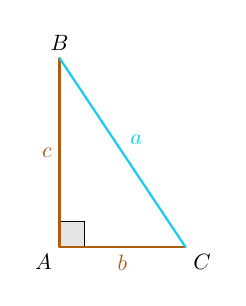
\begin{tikzpicture}[scale=0.8,transform shape]
   \tkzDefPoints{0/0/a,0/3/b,2/0/c}

   \tkzLabelPoint[below left](a){$A$}
   \tkzLabelPoint[above](b){$B$}
   \tkzLabelPoint[below right](c){$C$}

   \tkzLabelSegment[PolygonOrange,pos=0.5,left](a,b){$c$}
   \tkzLabelSegment[PolygonOrange,pos=0.5,below](a,c){$b$}
   \tkzLabelSegment[PolygonCyan,pos=0.5,above right](b,c){$a$}

   \tkzMarkRightAngle[size=.4,fill=Gray!20](c,a,b)

   \tkzDrawSegment[thick,PolygonOrange](a,b)
   \tkzDrawSegment[thick,PolygonOrange](a,c)
   \tkzDrawSegment[thick,PolygonCyan](b,c)
  \end{tikzpicture}
 \end{center}

 The \clo{short sides} are called \emph{catheti} and the \clb{long side} is
 called \emph{hypothenuse}.
\end{frame}

\begin{frame}
 \frametitle{Right Triangle}
 \begin{center}
  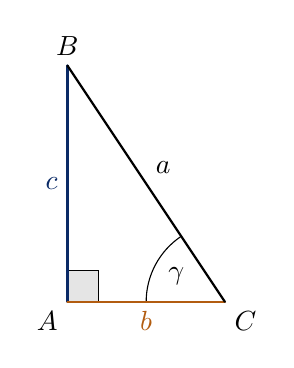
\begin{tikzpicture}
   \tkzDefPoints{0/0/a,0/3/b,2/0/c}

   \tkzLabelPoint[below left](a){$A$}
   \tkzLabelPoint[above](b){$B$}
   \tkzLabelPoint[below right](c){$C$}

   \tkzLabelSegment[PolygonBlue,pos=0.5,left](a,b){$c$}
   \tkzLabelSegment[PolygonOrange,pos=0.5,below](a,c){$b$}
   \tkzLabelSegment[pos=0.5,above right](b,c){$a$}

   \tkzMarkRightAngle[size=.4,fill=Gray!20](c,a,b)
   \tkzMarkAngle[size=1](b,c,a)
   \tkzLabelAngle[pos=0.7](b,c,a){$\gamma$}

   \tkzDrawSegment[thick,PolygonBlue](a,b)
   \tkzDrawSegment[thick,PolygonOrange](a,c)
   \tkzDrawSegment[thick](b,c)
  \end{tikzpicture}
 \end{center}
 With respect to a chosen angle $\gamma$, the side $\clb{c}$ is called
 \emph{opposite} and $\clo{b}$ is called \emph{adjacent}.
\end{frame}

\section{Pythagorean Theorem}

\begin{frame}
 \frametitle{Pythagorean Theorem}
 \begin{center}
  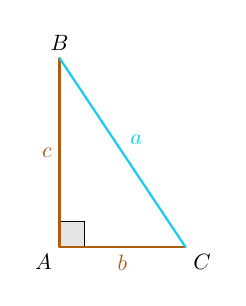
\begin{tikzpicture}[scale=0.8,transform shape]
   \tkzDefPoints{0/0/a,0/3/b,2/0/c}

   \tkzLabelPoint[below left](a){$A$}
   \tkzLabelPoint[above](b){$B$}
   \tkzLabelPoint[below right](c){$C$}

   \tkzLabelSegment[PolygonOrange,pos=0.5,left](a,b){$c$}
   \tkzLabelSegment[PolygonOrange,pos=0.5,below](a,c){$b$}
   \tkzLabelSegment[PolygonCyan,pos=0.5,above right](b,c){$a$}

   \tkzMarkRightAngle[size=.4,fill=Gray!20](c,a,b)

   \tkzDrawSegment[thick,PolygonOrange](a,b)
   \tkzDrawSegment[thick,PolygonOrange](a,c)
   \tkzDrawSegment[thick,PolygonCyan](b,c)
  \end{tikzpicture}
 \end{center}
 Given a right triangle, the \alert{Pythagorean Theorem} says that
 \[
  \clc{a^2} = \clo{b^2} + \clo{c^2}.
 \]
\end{frame}

\begin{frame}
 \frametitle{Pythagorean Theorem -- Proof}
 \begin{minipage}[t]{.49\textwidth}
  \begin{center}
   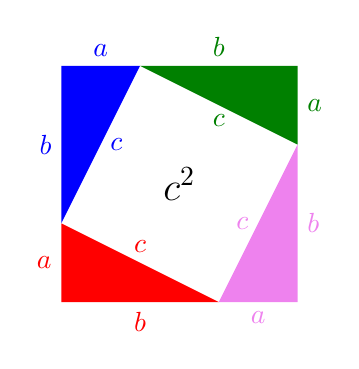
\begin{tikzpicture}
    \tkzDefPoints{0/0/a1,0/1/b1,2/0/c1}
    \tkzDefPoints{0/3/a2,1/3/b2,0/1/c2}
    \tkzDefPoints{3/3/a3,3/2/b3,1/3/c3}
    \tkzDefPoints{3/0/a4,2/0/b4,3/2/c4}

    \tkzDrawPolygon[fill=Red,draw=none](a1,b1,c1)
    \tkzDrawPolygon[fill=Blue,draw=none](a2,b2,c2)
    \tkzDrawPolygon[fill=Green,draw=none](a3,b3,c3)
    \tkzDrawPolygon[fill=Violet,draw=none](a4,b4,c4)

    \tkzLabelSegment[Red,left](a1,b1){$a$}
    \tkzLabelSegment[Red,below](a1,c1){$b$}
    \tkzLabelSegment[Red,above](b1,c1){$c$}

    \tkzLabelSegment[Blue,above](a2,b2){$a$}
    \tkzLabelSegment[Blue,left](a2,c2){$b$}
    \tkzLabelSegment[Blue,right](b2,c2){$c$}

    \tkzLabelSegment[Green,right](a3,b3){$a$}
    \tkzLabelSegment[Green,above](a3,c3){$b$}
    \tkzLabelSegment[Green,below](b3,c3){$c$}

    \tkzLabelSegment[Violet,below](a4,b4){$a$}
    \tkzLabelSegment[Violet,right](a4,c4){$b$}
    \tkzLabelSegment[Violet,left](b4,c4){$c$}

    \node (c) at (1.5,1.5) {\Large $c^2$};
   \end{tikzpicture}
  \end{center}
 \end{minipage}
 \pause
 \frametitle{Pythagorean Theorem -- Proof}
 \begin{minipage}[t]{.49\textwidth}
  \begin{center}
   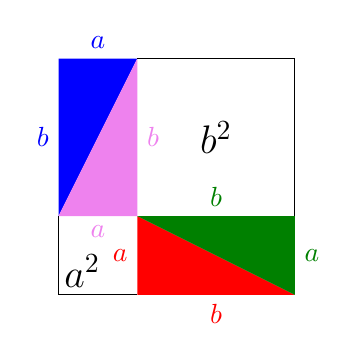
\begin{tikzpicture}
    \tkzDefPoints{0/3/a1,0/1/b1,1/3/c1,1/1/d1}
    \tkzDefPoints{1/0/a2,1/1/b2,3/0/c2,3/1/d2}

    \tkzDrawPolygon[fill=Blue,draw=none](a1,b1,c1)
    \tkzDrawPolygon[fill=Violet,draw=none](b1,c1,d1)
    \tkzDrawPolygon[fill=Red,draw=none](a2,b2,c2)
    \tkzDrawPolygon[fill=Green,draw=none](b2,c2,d2)

    \tkzLabelSegment[Blue,left](a1,b1){$b$}
    \tkzLabelSegment[Blue,above](a1,c1){$a$}
    \tkzLabelSegment[Violet,below](b1,d1){$a$}
    \tkzLabelSegment[Violet,right](c1,d1){$b$}

    \tkzLabelSegment[Red,left](a2,b2){$a$}
    \tkzLabelSegment[Red,below](a2,c2){$b$}
    \tkzLabelSegment[Green,above](b2,d2){$b$}
    \tkzLabelSegment[Green,right](c2,d2){$a$}

    \draw (c1.east) -- (3,3) -- (d2.north);
    \draw (b1.south) -- (0,0) -- (a2.west);

    \node (a^2) at (0.3,0.3) {\Large $a^2$};
    \node (b^2) at (2,2) {\Large $b^2$};
   \end{tikzpicture}
  \end{center}
 \end{minipage}
\end{frame}

\begin{frame}
 \frametitle{Pythagorean Theorem -- Problem 1}
 What is the length of the hypotenuse in a right triangle if the catheti are $5$
 and $12$?\\
 \pause
 We simply calculate ($h$ means hypotenuse)
 \begin{align*}
  h^2 &= 5^2 + 12^2 = 169\\
  h &= \sqrt{169} = 13.
 \end{align*}
\end{frame}

\begin{frame}
 \frametitle{Pythagorean Theorem -- Problem 2}
 Find the height of the following isosceles triangle:
 \begin{center}
  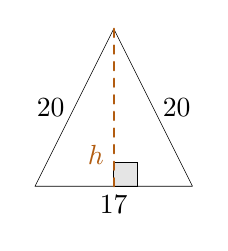
\begin{tikzpicture}
   \tkzDefPoints{0/0/mab,-1/0/a,1/0/b,0/2/c}
   \tkzMarkRightAngle[fill=gray!20,size=0.3](b,mab,c)
   \tkzDrawPolygon(a,b,c)
   \tkzLabelSegment(a,b){$17$}
   \tkzLabelSegment[left](a,c){$20$}
   \tkzLabelSegment[right](b,c){$20$}

   \tkzDrawSegment[thick,dashed,PolygonOrange](c,mab)
   \tkzLabelSegment[left,PolygonOrange,pos=0.8](c,mab){$h$}
  \end{tikzpicture}
  \vspace*{-1em}
 \end{center}
 \pause
 We have two right triangles next to each other -- each one with hypotenuse of
 length $20$ and one cathetus of length $17 / 2 = 8.5$.
 \pause
 So, we know that
 \[
  20^2 = 8.5^2 + \clo{h}^2,
 \]
 and thus $\clo{h}^2 = 20^2 - 8.5^2 = 327.75$ and $\clo{h} = \sqrt{327.75} =
 18.1$.
\end{frame}

\section{Applications}

\begin{frame}
 \frametitle{Architecture \& Construction}
 When constructing a roof, you typically only know the \clc{height} and
 \clo{width}.\\
 \pause 
 Using Pythagorean Theorem, you can also calculate the length of the diagonal
 slope and its area to cut out supporting beams.\\
 \pause
 For example, if the \clc{height} of the roof is 3 meters and its \clo{width} is
 6 meters,
 \begin{center}
  \begin{tikzpicture}[scale=0.75,transform shape]
   \tkzDefPoints{0/0/a,6/0/b,3/3/c}
   \tkzDrawSegment[PolygonCyan](a,b)
   \tkzLabelSegment[below,PolygonCyan](a,b){$w$}
   \tkzDefMidPoint(a,b) \tkzGetPoint{sab}
   \tkzDrawSegment[dashed,PolygonOrange](c,sab)
   \tkzLabelSegment[PolygonOrange,left](c,sab){$h$}
   \tkzDrawSegment(b,c)
   \tkzDrawSegment(a,c)
   \tkzLabelSegment[above right](b,c){$x$}
   \tkzLabelSegment[above left](a,c){$x$}
  \end{tikzpicture}
 \end{center}
 the length of the slope can be calculated as $x^2 = h^2 + (w / 2)^2 = 9 + 9 =
 18$ and taking the square root to get $x = 4.24$ meters.
\end{frame}

\begin{frame}
 \frametitle{Architecture \& Construction}
 A triangle with side lengths $a,b,c$ is a right triangle if and only if the
 Pythagorean Theorem $a^2 + b^2 = c^2$ holds.\\
 \pause
 This can be used to efficiently measure right angles. If we know, for instance,
 that a triangle with side lengths $3,4$ and $5$ is right, we can set out a
 triangle made of strings of these lengths to lay out a foundation or construct
 a corner between walls.\\
 \pause
 For example, one can make sure that the triangles of side lengths $5,12,13$ and
 $20,21,29$ are right because
 \begin{align*}
  5^2 + 12^2 &= 25 + 144 = 169 = 13^2,\\
  20^2 + 21^2 &= 400 + 441 = 841 = 29^2.
 \end{align*}
\end{frame}

\begin{frame}
 \frametitle{Navigation}
 The Pythagorean Theorem is useful when calculating distances between points in
 the plane or in space.\\
 For example, to calculate the distance between $(1,2)$ and $(3,5)$, one sets up
 a right triangle like this:
 \begin{center}
  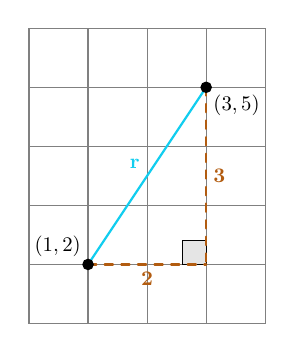
\begin{tikzpicture}[scale=0.75,transform shape]
   \tkzInit[xmin=0,xmax=4,ymin=1,ymax=6]
   \tkzGrid
   \tkzDefPoints{1/2/x,3/5/y,3/2/z}
   \tkzDrawSegment[thick,PolygonCyan](x,y)
   \tkzMarkRightAngle[size=.4,fill=Gray!20](y,z,x)
   \tkzLabelPoint[above left](x){$(1,2)$}
   \tkzLabelPoint[below right](y){$(3,5)$}
   \tkzLabelSegment[PolygonCyan,above left](x,y){$\mathbf{r}$}
   \tkzDrawSegment[thick,dashed,PolygonOrange](y,z)
   \tkzDrawSegment[thick,dashed,PolygonOrange](x,z)
   \tkzLabelSegment[PolygonOrange,right](y,z){$\mathbf{3}$}
   \tkzLabelSegment[PolygonOrange,below](x,z){$\mathbf{2}$}
   \tkzDrawPoints(x,y)
  \end{tikzpicture}
 \end{center}
\end{frame}

\begin{frame}
 \frametitle{Navigation}
 \begin{center}
  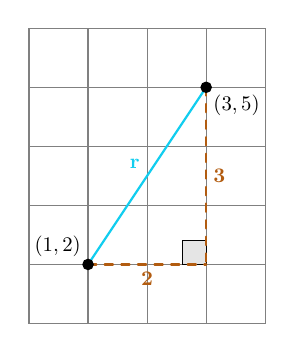
\begin{tikzpicture}[scale=0.75,transform shape]
   \tkzInit[xmin=0,xmax=4,ymin=1,ymax=6]
   \tkzGrid
   \tkzDefPoints{1/2/x,3/5/y,3/2/z}
   \tkzDrawSegment[thick,PolygonCyan](x,y)
   \tkzMarkRightAngle[size=.4,fill=Gray!20](y,z,x)
   \tkzLabelPoint[above left](x){$(1,2)$}
   \tkzLabelPoint[below right](y){$(3,5)$}
   \tkzLabelSegment[PolygonCyan,above left](x,y){$\mathbf{r}$}
   \tkzDrawSegment[thick,dashed,PolygonOrange](y,z)
   \tkzDrawSegment[thick,dashed,PolygonOrange](x,z)
   \tkzLabelSegment[PolygonOrange,right](y,z){$\mathbf{3}$}
   \tkzLabelSegment[PolygonOrange,below](x,z){$\mathbf{2}$}
   \tkzDrawPoints(x,y)
  \end{tikzpicture}
 \end{center}
 So, the distance from $(1,2)$ to $(3,5)$ satisfies
 \begin{align*}
  \clc{r}^2 &= 2^2 + 3^2,\\
  \clc{r} &= \sqrt{13}.
 \end{align*}
\end{frame}

\begin{frame}
 \frametitle{Navigation}
 Distances in 3D are measured the same way, one just has to set up two right
 triangles.\\
 \pause
 For example, let's measure the distance from $(1,0,2)$ to $(3,3,3)$. We set up
 our right triangles:
 \begin{center}
  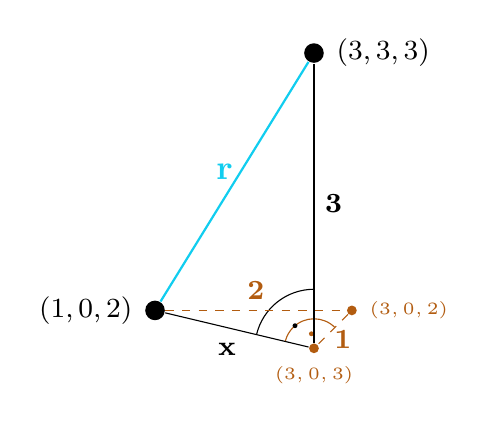
\begin{tikzpicture}[scale=1.25,transform shape]
   \node[circle,fill,inner sep=2pt] (x) at (1,0,2) {};
   \node[circle,fill,inner sep=2pt] (y) at (3,3,3){};
   \node[circle,fill,inner sep=1pt,PolygonOrange] (z1) at (3,0,2) {};
   \node[circle,fill,inner sep=1pt,PolygonOrange] (z2) at (3,0,3) {};

   \node[left=0mm of x] {\footnotesize $(1,0,2)$};
   \node[right=0mm of y] {\footnotesize $(3,3,3)$};

   \node[below=0mm of z2,PolygonOrange] {\tiny $(3,0,3)$};
   \node[right=0mm of z1,PolygonOrange] {\tiny $(3,0,2)$};
   
   \pic [draw=PolygonOrange,angle radius=3mm] {angle = z1--z2--x};
   \pic [draw=black,angle radius=6mm] {angle = y--z2--x};
   \node[circle,fill,inner sep=.5pt,PolygonOrange] at ($(z2) + (100:0.15)$) {};
   \node[circle,fill,inner sep=.5pt] at ($(z2) + (130:0.3)$) {};

   \draw (x) to node[midway,xshift=-1mm,yshift=-2mm]{\footnotesize $\mathbf{x}$}
    (z2);
   \draw (z2) to node[midway,xshift=2mm]{\footnotesize $\mathbf{3}$} (y);
   \draw[dashed,PolygonOrange] (x) to
    node[midway,PolygonOrange,yshift=2mm]{\footnotesize $\mathbf{2}$} (z1);
   \draw[dashed,PolygonOrange] (z1) to
    node[midway,PolygonOrange,xshift=1mm,yshift=-1mm]{\footnotesize $\mathbf{1}$} (z2);
   \draw[thick,PolygonCyan] (x) to
    node[midway,PolygonCyan,xshift=-1mm,yshift=1mm]{\clc{\textbf{r}}} (y);
  \end{tikzpicture}
 \end{center}
\end{frame}

\begin{frame}
 \frametitle{Navigation}
 \begin{center}
  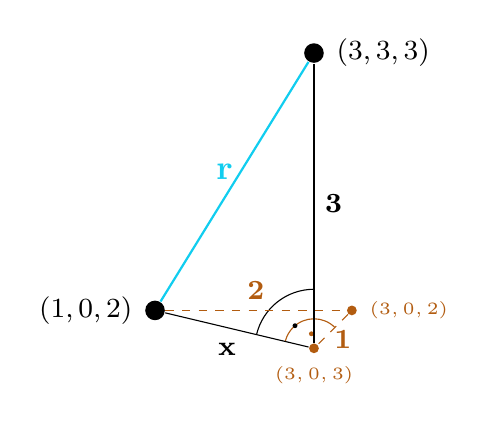
\begin{tikzpicture}[scale=1.25,transform shape]
   \node[circle,fill,inner sep=2pt] (x) at (1,0,2) {};
   \node[circle,fill,inner sep=2pt] (y) at (3,3,3){};
   \node[circle,fill,inner sep=1pt,PolygonOrange] (z1) at (3,0,2) {};
   \node[circle,fill,inner sep=1pt,PolygonOrange] (z2) at (3,0,3) {};

   \node[left=0mm of x] {\footnotesize $(1,0,2)$};
   \node[right=0mm of y] {\footnotesize $(3,3,3)$};

   \node[below=0mm of z2,PolygonOrange] {\tiny $(3,0,3)$};
   \node[right=0mm of z1,PolygonOrange] {\tiny $(3,0,2)$};

   \pic [draw=PolygonOrange,angle radius=3mm] {angle = z1--z2--x};
   \pic [draw=black,angle radius=6mm] {angle = y--z2--x};
   \node[circle,fill,inner sep=.5pt,PolygonOrange] at ($(z2) + (100:0.15)$) {};
   \node[circle,fill,inner sep=.5pt] at ($(z2) + (130:0.3)$) {};

   \draw (x) to node[midway,xshift=-1mm,yshift=-2mm]{\footnotesize $\mathbf{x}$}
    (z2);
   \draw (z2) to node[midway,xshift=2mm]{\footnotesize $\mathbf{3}$} (y);
   \draw[dashed,PolygonOrange] (x) to
    node[midway,PolygonOrange,yshift=2mm]{\footnotesize $\mathbf{2}$} (z1);
   \draw[dashed,PolygonOrange] (z1) to
    node[midway,PolygonOrange,xshift=1mm,yshift=-1mm]{\footnotesize $\mathbf{1}$} (z2);
   \draw[thick,PolygonCyan] (x) to
    node[midway,PolygonCyan,xshift=-1mm,yshift=1mm]{\clc{\textbf{r}}} (y);
   
  \end{tikzpicture}
 \end{center}
 \vspace*{-1em}
 From this, we can calculate
 \[
  x = \sqrt{1^2 + 2^2} = \sqrt{5}, \quad 
  \clc{r} = \sqrt{3^2 + (\sqrt{5})^2} = \sqrt{9 + 5} = \sqrt{14}.
 \]
\end{frame}

\end{document}
